\section{Validation}\label{sec:valid}
In the scope of this thesis a program was developed that implements flat shell elements. Two different discretizations of shell elements are provided: A three-node triangular element and a four-node quadrilateral element. A plane and a plate bending element were superimposed to the final flat shell element. This chapter attends the validation, i.e. the accuracy and convergence properties, of the two shell element discretizations as well as their parts, the plane and the plate element. Several problems were chosen that show the correctness of the discretized elements. The tests were taken from different sources, namely \cite{kansara2004development}, \cite{macneal1985proposed}, \cite{wilson1996three} and \cite{jin1994analysis}. Many example problems have analytical results to be compared with, the examples from \cite{kansara2004development} used a commercial software called \textit{SAP2000} \cite{sap-2000} as a benchmark for comparison. Since this software is used in practice for over 30 years, it will be used here as a benchmark as well.
 \subsection{Test A: Plane Displacement with Tri-3 Element}\label{sec:valid-A}
  The three-node triangular plane element \textbf{Tri-3} is validated with a cantilever beam shown in Figure \ref{fig:testA}. The example problem was taken from \cite{kansara2004development} (Test Example 2).
 \begin{figure}[htbp]
   	\centering
	\setlength\unitlength{1.65cm}
   	\begin{picture}(9,3)
   	\thicklines
   	\put(4.51,1.51){\vector(1,0){0.75}}
   	\put(4.52,1.5){\vector(0,1){0.75}}
   	\put(5.07,1.27){$\mathbf{x}$}
   	\put(4.55,2.13){$\mathbf{y}$}   	
   	\put(8.52,0.0){\vector(0,1){0.5}}
   	\put(8.52,1.0){\vector(0,1){0.5}}
   	\put(8.52,2.0){\vector(0,1){0.5}}   	
   	\thinlines
   	\polygon(0.5,0.5)(0.5,2.5)(8.5,2.5)(8.5,0.5)
   	\polyline(0.5,1.5)(1.5,2.5)(1.5,0.5)(0.5,1.5)(1.5,1.5)
   	\polyline(1.5,1.5)(2.5,2.5)(2.5,0.5)(1.5,1.5)(2.5,1.5)
   	\polyline(2.5,1.5)(3.5,2.5)(3.5,0.5)(2.5,1.5)(3.5,1.5)
   	\polyline(3.5,1.5)(4.5,2.5)(4.5,0.5)(3.5,1.5)(4.5,1.5)
   	\polyline(4.5,1.5)(5.5,2.5)(5.5,0.5)(4.5,1.5)(5.5,1.5)
   	\polyline(5.5,1.5)(6.5,2.5)(6.5,0.5)(5.5,1.5)(6.5,1.5)
   	\polyline(6.5,1.5)(7.5,2.5)(7.5,0.5)(6.5,1.5)(7.5,1.5)
   	\polyline(7.5,1.5)(8.5,2.5)(8.5,0.5)(7.5,1.5)(8.5,1.5)   	
   	\Line(0.5,0.5)(0.3,0.7) \Line(0.5,1)(0.3,1.2) \Line(0.5,1.5)(0.3,1.7) \Line(0.5,2)(0.3,2.2) \Line(0.5,2.5)(0.3,2.7)   	
   	\put(8.6,0.15){$6\frac{2}{3}$}
   	\put(8.6,1.15){$26\frac{2}{3}$}
   	\put(8.6,2.15){$6\frac{2}{3}$}   	
   	\put(0.56,0.55){$0$} \put(1.56,0.55){$1$} \put(2.56,0.55){$2$} \put(3.56,0.55){$3$} \put(4.56,0.55){$4$} \put(5.56,0.55){$5$} \put(6.56,0.55){$6$} \put(7.56,0.55){$7$} \put(8.56,0.55){$8$}
   	\put(0.56,1.55){$9$}  \put(1.56,1.55){$10$} \put(2.56,1.55){$11$} \put(3.56,1.55){$12$} \put(4.56,1.55){$13$} \put(5.56,1.55){$14$} \put(6.56,1.55){$15$} \put(7.56,1.55){$16$} \put(8.56,1.55){$17$}
   	\put(0.56,2.55){$18$} \put(1.56,2.55){$19$} \put(2.56,2.55){$20$} \put(3.56,2.55){$21$} \put(4.56,2.55){$22$} \put(5.56,2.55){$23$} \put(6.56,2.55){$24$} \put(7.56,2.55){$25$} \put(8.56,2.55){$26$}
   	\end{picture}
   	\caption{Cantilever beam consisting of 32 triangular elements, clamped at the left side and a total force of 40 kips applied in positive y-direction at the right side}
   	\label{fig:testA}
   \end{figure}
      
   \begin{itemize}
   \item \textbf{Mesh dimensions}\\
   Length $l = 48\ inch$\\
   Depth $h = 12\ inch$\\
   Thickness $t = 1\ inch$
   
   \item \textbf{Material properties}\\
   Young's Modulus $E = 30000 ksi$\\
   Poisson's ratio $\nu = 0.25$
   
   \item \textbf{Boundary conditions}\\
   Clamped boundary conditions at node 0, 9 and 18, i.e.\ left side of the cantilever beam.
   
   \item \textbf{Loading}\\
   A concentrated load of $40 kips$ in total. Node 8 and 26 has a load of $6 \frac{2}{3}$, node 17 has a load of $26 \frac{2}{3}$.
   \end{itemize}
   
   \paragraph{Results:} The displacements in x- and y-direction at node 22 and 26 are presented in Table \ref{tab:testA} together with the results from the \textit{SAP2000} software presented in \cite{kansara2004development}. The displacements of the thesis' program deviate from the commercial software in all cases for at most $0.027\%$. The triangle orientation in the example mesh contains both, the square diagonal facing the upper right and facing the lower right corner of the square. To show that the mixed usage of these orientation types increases the accuracy, two additional tests were made, one with only triangles having their hypotenuse facing the upper right corner of the square ($\boxslash$) and one with only triangles of the other type ($\boxbackslash$). The results of those tests can only be compared to the first test's results of the program, since no benchmark values are available. What can first be seen is that either of the new variants is less accurate than the mixed version. Second, the $\boxslash$-variant is more accurate than the $\boxbackslash$-variant and third, the accuracy in x-direction is better than in y-direction, particularly for the $\boxbackslash$-orientation.
   
   \begin{table}[htbp]
   \centering
   \begin{tabular}{c|c|C{2.5cm}|C{2.5cm}|c}
   \textbf{Node} & \textbf{Displacement} & \textbf{Results from program$^{(a)}$} & \textbf{Results from SAP2000$^{(b)}$} & \textbf{Difference (\%)}\\\hline\hline
   \multirow{2}{*}{22} & $u_x$ & $-0.0255988$ & $-0.025605$ & $0.024\%^{(b)}$\\
                       & $u_y$ & $ 0.0629549$ & $ 0.062971$ & $0.026\%^{(b)}$\\\hline
   \multirow{2}{*}{26} & $u_x$ & $-0.0342621$ & $-0.034271$ & $0.027\%^{(b)}$\\
                       & $u_y$ & $ 0.1944070$ & $ 0.194456$ & $0.025\%^{(b)}$\\\hline\hline
   \multirow{2}{*}{$\boxslash$ 22}     & $u_x$ & $-0.0243863$ & - & $4.97\%^{(a)}$\\
                                         & $u_y$ & $ 0.0552195$ & - & $14.01\%^{(a)}$\\\hline
   \multirow{2}{*}{$\boxslash$ 26}     & $u_x$ & $-0.0328891$ & - & $4.17\%^{(a)}$\\
                                         & $u_y$ & $ 0.1829420$ & - & $6.27\%^{(a)}$\\\hline\hline
   \multirow{2}{*}{$\boxbackslash$ 22} & $u_x$ & $-0.0235617$ & - & $8.65\%^{(a)}$\\
                                         & $u_y$ & $ 0.0440028$ & - & $43.07\%^{(a)}$\\\hline
   \multirow{2}{*}{$\boxbackslash$ 26} & $u_x$ & $-0.0322955$ & - & $6.09\%^{(a)}$\\
                                         & $u_y$ & $ 0.1564130$ & - & $24.29\%^{(a)}$\\\hline
   \end{tabular}
   \caption{Displacements and deviations for Test A}
   \label{tab:testA}
   \end{table}
   
   
 \subsection{Test B: Plane Displacement with Quad-4}\label{sec:valid-B}
  The four-node quadrilateral plane element \textbf{Quad-4} is validated with the same cantilever beam that was used in Test A. It is shown in Figure \ref{fig:testB}. The example problem was also taken from \cite{kansara2004development} (Test Example 5).
  \begin{figure}[htbp]
    \centering
  	\setlength\unitlength{1.65cm}
   	\begin{picture}(9,3)
   	\thicklines
   	\put(4.51,1.51){\vector(1,0){0.75}}
   	\put(4.52,1.5){\vector(0,1){0.75}}
   	\put(5.07,1.27){$\mathbf{x}$}
   	\put(4.55,2.13){$\mathbf{y}$}   	
   	\put(8.52,0.0){\vector(0,1){0.5}}
   	\put(8.52,1.0){\vector(0,1){0.5}}
   	\put(8.52,2.0){\vector(0,1){0.5}}   	
   	\thinlines
   	\polygon(0.5,0.5)(0.5,2.5)(8.5,2.5)(8.5,0.5)
   	\Line(0.5,1.5)(8.5,1.5)
   	\Line(1.5,0.5)(1.5,2.5) \Line(2.5,0.5)(2.5,2.5) \Line(3.5,0.5)(3.5,2.5) \Line(4.5,0.5)(4.5,2.5) \Line(5.5,0.5)(5.5,2.5) \Line(6.5,0.5)(6.5,2.5) \Line(7.5,0.5)(7.5,2.5)
   	\Line(0.5,0.5)(0.3,0.7) \Line(0.5,1)(0.3,1.2) \Line(0.5,1.5)(0.3,1.7) \Line(0.5,2)(0.3,2.2) \Line(0.5,2.5)(0.3,2.7)   	
   	\put(8.6,0.15){$6\frac{2}{3}$}
   	\put(8.6,1.15){$26\frac{2}{3}$}
   	\put(8.6,2.15){$6\frac{2}{3}$}   	
   	\put(0.56,0.55){$0$} \put(1.56,0.55){$1$} \put(2.56,0.55){$2$} \put(3.56,0.55){$3$} \put(4.56,0.55){$4$} \put(5.56,0.55){$5$} \put(6.56,0.55){$6$} \put(7.56,0.55){$7$} \put(8.56,0.55){$8$}
   	\put(0.56,1.55){$9$}  \put(1.56,1.55){$10$} \put(2.56,1.55){$11$} \put(3.56,1.55){$12$} \put(4.56,1.55){$13$} \put(5.56,1.55){$14$} \put(6.56,1.55){$15$} \put(7.56,1.55){$16$} \put(8.56,1.55){$17$}
   	\put(0.56,2.55){$18$} \put(1.56,2.55){$19$} \put(2.56,2.55){$20$} \put(3.56,2.55){$21$} \put(4.56,2.55){$22$} \put(5.56,2.55){$23$} \put(6.56,2.55){$24$} \put(7.56,2.55){$25$} \put(8.56,2.55){$26$}
   	\end{picture}
   	\caption{Cantilever beam consisting of 16 quadrilateral elements, clamped at the left side and a total force of 40 kips applied in positive y-direction at the right side}
   	\label{fig:testB}
  \end{figure}

  \begin{itemize}
   \item \textbf{Mesh dimensions}\\
   Length $l = 48\ inch$\\
   Depth $h = 12\ inch$\\
   Thickness $t = 1\ inch$

   \item \textbf{Material properties}\\
   Young's Modulus $E = 30000 ksi$\\
   Poisson's ratio $\nu = 0.25$

   \item \textbf{Boundary conditions}\\
   Clamped boundary conditions at node 0, 9 and 18, i.e.\ left side of the cantilever beam.

   \item \textbf{Loading}\\
   A concentrated load of $40 kips$ in total. Node 8 and 26 has a load of $6 \frac{2}{3}$, node 17 has a load of $26 \frac{2}{3}$.
  \end{itemize}

  \paragraph{Results:} The displacements in x- and y-direction at node 22 and 26 are presented in Table \ref{tab:testB}. The results of \textit{SAP2000} were used for comparison. The displacements calculated by the thesis' program deviate from the commercial software in all cases for at most $0.03\%$ and thus can be accepted as satisfactory accurate.

  \begin{table}[htbp]
   \centering
    \begin{tabular}{c|c|C{2.5cm}|C{2.5cm}|c}
    \textbf{Node} & \textbf{Displacement} & \textbf{Results from program} & \textbf{Results from SAP-2000} & \textbf{Difference (\%)}\\\hline\hline
    \multirow{2}{*}{22} & $u_x$ & $-0.0427728$ & $-0.042774$ & $0.028\%$\\
                        & $u_y$ & $ 0.1012620$ & $ 0.101265$ & $0.030\%$\\\hline
    \multirow{2}{*}{26} & $u_x$ & $-0.0570728$ & $-0.057074$ & $0.021\%$\\
                        & $u_y$ & $ 0.3160560$ & $ 0.316064$ & $0.025\%$\\\hline
    \end{tabular}
   \caption{Displacements and deviations for Test B}
   \label{tab:testB}
   \end{table}
     
 \subsection{Test C: Plate Displacement with Tri-3}\label{sec:valid-C}
  In this test the three-node triangular plate element \textbf{Tri-3} was validated. The example problem was taken from \cite{wilson1996three} (8.9.2). The geometry of the test is shown in Figure \ref{fig:testC}. Four different tests were made: At first the square plate were subdivided into $4\!\times\!4$ squares. Each square were divided into two triangles by a diagonal. Here, two possibilities are given: From the upper left to the lower right ($\boxbackslash$) or from the upper right to the lower left ($\boxslash$). This variant is shown in Figure \ref{fig:testC}. The other two tests were made with the same triangle variants but with a $16\!\times\!16$ mesh subdivision.
  \begin{figure}[htbp]
  	\centering
  	\setlength\unitlength{1.05cm}
  	\begin{picture}(7,7.5)
  	\thicklines
  	\put(0.5,0.5){\vector(1,0){1}}
  	\put(0.5,0.5){\vector(0,1){1}}
  	\put(1.6,0.6){$\mathbf{x}$}
  	\put(0.6,1.6){$\mathbf{y}$}   	
  	\thinlines
  	\polygon(1,1)(7,1)(7,7)(1,7)
  	\Line(1,4)(7,4)\Line(4,1)(4,7)
  	\Line(1,2.5)(7,2.5)\Line(2.5,1)(2.5,7)
  	\Line(1,5.5)(7,5.5)\Line(5.5,1)(5.5,7)
  	\Line(1,1)(7,7)\Line(1,2.5)(5.5,7)\Line(1,4)(4,7)\Line(1,5.5)(2.5,7)\Line(2.5,1)(7,5.5)\Line(4,1)(7,4)\Line(5.5,1)(7,2.5)
  	\polygon(1,1)(1.1,0.8)(0.9,0.8)
  	\polygon(1,1)(0.8,1.1)(0.8,0.9)
  	\polygon(7,1)(7.1,0.8)(6.9,0.8)
  	\polygon(7,1)(7.2,1.1)(7.2,0.9)
  	\polygon(7,7)(7.1,7.2)(6.9,7.2)
  	\polygon(7,7)(7.2,7.1)(7.2,6.9)
  	\polygon(1,7)(1.1,7.2)(0.9,7.2)
  	\polygon(1,7)(0.8,7.1)(0.8,6.9)
  	\put(4,4){\circle*{0.25}} \put(4.1,3.65){$P$}
  	\put(1.06,1.05){$0$}\put(2.56,1.05){$1$}\put(4.06,1.05){$2$}\put(5.56,1.05){$3$}\put(7.06,1.05){$4$}
  	\put(1.06,2.55){$5$}\put(2.56,2.55){$6$}\put(4.06,2.55){$7$}\put(5.56,2.55){$8$}\put(7.06,2.55){$9$}
  	\put(1.06,4.05){$10$}\put(2.56,4.05){$11$}\put(4.06,4.05){$12$}\put(5.56,4.05){$13$}\put(7.06,4.05){$14$}
  	\put(1.06,5.55){$15$}\put(2.56,5.55){$16$}\put(4.06,5.55){$17$}\put(5.56,5.55){$18$}\put(7.06,5.55){$19$}
  	\put(1.06,7.05){$20$}\put(2.56,7.05){$21$}\put(4.06,7.05){$22$}\put(5.56,7.05){$23$}\put(7.06,7.05){$24$}
  	\end{picture}
  	\caption{A square plate simply supported on all four sides is shown with a mesh subdivision of $4\!\times\!4$ squares. Each square is divided into two triangles through a diagonal going from the lower left to the upper right corner. This orientation is symbolized by ``$\boxslash$''. In the center of the plate a concentrated load $P$ is applied.}
  	\label{fig:testC}
  \end{figure}
  
  \begin{itemize}
  	\item \textbf{Mesh dimensions}\\
  	Side length $l = 10.0$\\
  	Thickness $t = 1.0$
  	
  	\item \textbf{Material properties}\\
  	Young's Modulus $E = 10.92$\\
  	Poisson's ratio $\nu = 0.3$
  	
  	\item \textbf{Boundary conditions}\\
  	All sides of the square plate are simply supported.
  	
  	\item \textbf{Loading}\\
  	A concentrated load of $1.0$ is applied on the center node of the square.
  \end{itemize}
  
  \paragraph{Results:} Wilson \cite{wilson1996three} states that the exact thin-plate displacement of the central node for this problem is $w_c = 1.16$. The results of the test is presented in Table \ref{tab:testC}. The program's result is compared to the exact value as well as to the results of the Dircrete Kirchhoff Element (DKE) presented in \cite{wilson1996three}. The DKE is also a three-node triangular plate bending element. At first, the results show that no difference exists between the different orientations of the triangles. For the $4\!\times\!4$ mesh subdivision the difference between the program's result and the benchmark is $10.69\%$ while it is only $8.69\%$ compared with the exact value. The relative big difference can be explained by the simple formulation of the Tri-3 element. For the $16\!\times\!16$ mesh subdivision the difference shrinks to only $0.72\%$ compared to the exact value and $0.97\%$ to the benchmark.  
  \begin{table}[htbp]
  	\centering
  	\begin{tabular}{C{1.5cm}|C{3.0cm}|C{2.5cm}|C{2.5cm}|C{2.7cm}}
\small\textbf{Mesh variant} & \small\textbf{Displacement at center node} & \small\textbf{Results from program} & \small\textbf{Results of DKE} & \small\textbf{Difference to 1.16 (\%)}\\\hline\hline
\multicolumn{5}{l}{$4\!\times\!4$ mesh subdivision}\\\hline
$\boxslash$     & $w_{c_{12}}$ & $1.06723$ & $1.195$ & $8.69\%$\\\hline
$\boxbackslash$ & $w_{c_{12}}$ & $1.06723$ & $1.195$ & $8.69\%$\\\hline\hline
\multicolumn{5}{l}{$16\!\times\!16$ mesh subdivision}\\\hline
$\boxslash$     & $w_{c_{144}}$ & $1.15169$ & $1.163$ & $0.72\%$\\\hline
$\boxbackslash$ & $w_{c_{144}}$ & $1.15169$ & $1.163$ & $0.72\%$\\\hline
  	\end{tabular}
  	\caption{Displacements and deviations for Test C}
  	\label{tab:testC}
  \end{table}
 \subsection{Test D: Plate Displacement with Quad-4}\label{sec:valid-D}
 This example problem tests the four-node quadrilateral plate element \textbf{Quad-4}. The test was taken from \cite{jin1994analysis} (4.2.1, 4.2.2). Several different configurations were made: The square plate was subdivided into 4, 8 and 16 square elements on each direction. Each mesh subdivision was then tested with a concentrated load of 30000 on the central node and with a uniformly distributed load of 300 per square unit. The geometry of for one of the six test configurations is shown in Figure \ref{fig:testD}.
  \begin{figure}[htbp]
  	\centering
  	\setlength\unitlength{1.05cm}
  	\begin{picture}(8,8)
  	\thicklines
  	\put(0.5,0.5){\vector(1,0){1}}
  	\put(0.5,0.5){\vector(0,1){1}}
  	\put(1.6,0.6){$\mathbf{x}$}
  	\put(0.6,1.6){$\mathbf{y}$}   	
  	\thinlines
  	\polygon(1,1)(7,1)(7,7)(1,7)
  	\Line(1,1.75)(7,1.75)\Line(1.75,1)(1.75,7)
  	\Line(1,2.50)(7,2.50)\Line(2.50,1)(2.50,7)
  	\Line(1,3.25)(7,3.25)\Line(3.25,1)(3.25,7)
  	\Line(1,4.00)(7,4.00)\Line(4.00,1)(4.00,7)
  	\Line(1,4.75)(7,4.75)\Line(4.75,1)(4.75,7)  	
  	\Line(1,5.50)(7,5.50)\Line(5.50,1)(5.50,7)
	\Line(1,6.25)(7,6.25)\Line(6.25,1)(6.25,7)
  	\polygon(1,1)(1.1,0.8)(0.9,0.8)
  	\polygon(1,1)(0.8,1.1)(0.8,0.9)
  	\polygon(7,1)(7.1,0.8)(6.9,0.8)
  	\polygon(7,1)(7.2,1.1)(7.2,0.9)
  	\polygon(7,7)(7.1,7.2)(6.9,7.2)
  	\polygon(7,7)(7.2,7.1)(7.2,6.9)
  	\polygon(1,7)(1.1,7.2)(0.9,7.2)
  	\polygon(1,7)(0.8,7.1)(0.8,6.9)
  	\put(4,4){\circle*{0.25}} \put(4.1,3.65){$P$}
  	\put(1.06,1.05){$0$}\put(4.06,1.05){$4$}\put(7.06,1.05){$8$}
  	\put(1.06,2.55){$18$}\put(4.06,2.55){$22$}\put(7.06,2.55){$26$}
  	\put(1.06,4.05){$36$}\put(4.06,4.05){$40$}\put(7.06,4.05){$44$}
  	\put(1.06,5.55){$54$}\put(4.06,5.55){$58$}\put(7.06,5.55){$62$}
  	\put(1.06,7.05){$72$}\put(4.06,7.05){$76$}\put(7.06,7.05){$80$}
  	\end{picture}
  	\caption{The mesh of test D is shown with a $8\!\times\!8$ subdivision and concentrated central loading configuration. The mesh can be subdivided coarser of finer and the loading can be applied uniformly over the whole plate. The square plate is in all cases simply supported on all four sides.}
  	\label{fig:testD}
  \end{figure}
  
  \begin{itemize}
   \item \textbf{Mesh dimensions}\\
   Side length $l = 10.0$\\
   Thickness $t = 0.5$
    	
   \item \textbf{Material properties}\\
   Young's Modulus $E = 10^7$\\
   Poisson's ratio $\nu = 0.3$
    	
   \item \textbf{Boundary conditions}\\
   All sides of the square plate are simply supported.
    	
   \item \textbf{Loading}\\
   A uniform load of $300$ is applied on the whole plate in a first test, while a concentrated load of $30,000$ is applied on the center node of the square in a second test.
  \end{itemize}
    
  \paragraph{Results:} For the test with the uniform load, \cite{jin1994analysis} states that the displacement of the central node $w_c^*$ can be evaluated exactly with the help of the plate theory, that is:
  \begin{equation}\label{eq:test-WC*q}
  w_c^* = \alpha \frac{q_0 a^4}{D}
  \end{equation}
  With $\alpha = 0.00406$ and $q_0 = 300$ being the uniform load, $a = 10$ the length of the square plate and $D = \frac{E t^3}{12 (1-\nu^2)}$ the material property, the central node's displacement follows as:
  \begin{equation*}
  w_c^* = 0.00406 \frac{300 * 10^4}{\frac{10^7 0.5^3}{12(1-0.3^2)}} = 0.1064045
  \end{equation*}
  The results with the different mesh subdivision levels are very accurate, the $8\!\times\!8$-subdivision if less than a thousands percents different to the analytical solution and even the coarse level with only 4 elements per direction has only $0.35\%$ difference to the exact value.\\
  For the concentrated load test, \cite{jin1994analysis} also proposes an analytic solution, namely:
  \begin{equation}\label{eq:test-WC*P}
  w_c^* = \alpha \frac{P a^2}{D}
  \end{equation}
  where $\alpha = 0.0115999$ and $P = 30000$ is the concentrated load at the center node. The rest of the variables stays the same as in the uniform load test. The analytical solution to this example problem is then $
  w_c^* = 0.30401019$. The program's results are far more inaccurate compared to the uniform load test with a maximum difference of $8.62\%$. The fine subdivision of $16\!\times\!16$ elements is though acceptably accurate with less than a percent difference to the analytically exact value.
  \begin{table}[htbp]
   \centering
   \begin{tabular}{C{2.0cm}|C{3.0cm}|C{2.5cm}|C{2.5cm}|C{2.7cm}}
\small\textbf{Mesh subdivisions} & \small\textbf{Displacement at center node} & \small\textbf{Results from program} & \small\textbf{Analytical solution} & \small\textbf{Difference (\%)}\\\hline\hline
  \multicolumn{5}{l}{Uniform loading}\\\hline
  $4\!\times\!4$   & $w_{c_{12}}$ & $0.106032$ & \multirow{3}{*}{$0.1064045$} & $0.35\%$\\\cline{1-3}\cline{5-5}
  $8\!\times\!8$   & $w_{c_{40}}$ & $0.106405$ &  & $0.00047\%$\\\cline{1-3}\cline{5-5}
  $16\!\times\!16$ & $w_{c_{144}}$& $0.106454$ &  & $0.046\%$\\\hline\hline
  \multicolumn{5}{l}{Concentrated loading}\\\hline
  $4\!\times\!4$   & $w_{c_{12}}$ & $0.332677$ & \multirow{3}{*}{$0.30401019$} & $8.62\%$\\\cline{1-3}\cline{5-5}
  $8\!\times\!8$   & $w_{c_{40}}$ & $0.312851$ &  & $2.83\%$\\\cline{1-3}\cline{5-5}
  $16\!\times\!16$ & $w_{c_{144}}$& $0.306664$ &  & $0.86\%$\\\hline
    	\end{tabular}
    	\caption{Displacements and deviations for Test D}
    	\label{tab:testD}
    \end{table}
 \subsection{Test E: Shell Displacement}\label{sec:valid-E}
 In Test A to D the single components of the Tri-3 and Quad-4 flat shell elements were validated. This test shows the accuracy of the shell elements by an example problem taken from \cite{kansara2004development} (Test Example 13 and 17). An I-beam is clamped on one end while loads are applied at the flanges of the other end's corners. Figure \ref{fig:testE} shows details on the geometry. The force causes the beam to get twisted around the global x-axis. The I-beam will have deformations in every direction for which shell elements are needed. The Tri-3 element is validated as well as the Quad-4 with the same geometry and load configuration.
 \begin{figure}[htbp]
  \centering
  \setlength\unitlength{1.00cm}
  \begin{picture}(12.5,5.5)
   \thicklines
   \polyline(2,1.0625)(0.5,0.5)(3.5,0.5)(11.5,3.5)(10,3.5)(10,4.4375)
   \polyline(2,0.5)(2,2)(3.5,2)(11.5,5)(8.5,5)(0.5,2)(2,2)
   \put(12.1,3.5){\vector(-1,0){0.6}}
   \put(7.9,5){\vector(1,0){0.6}}
   
   \put(10,0.5){\vector(0,1){1}}\put(9.9,1.6){$z$}
   \put(10,0.5){\vector(1,0){1}}\put(11.1,0.4){$y$}
   \put(10,0.5){\vector(8,3){1}}\put(11.1,0.9){$x$}
   
   \Line(0.85,0.5)(0.75,0.25)\Line(1.1,0.5)(1,0.25)\Line(1.35,0.5)(1.25,0.25)\Line(1.6,0.5)(1.5,0.25)\Line(1.85,0.5)(1.75,0.25)\Line(2.35,0.5)(2.25,0.25)\Line(2.6,0.5)(2.5,0.25)\Line(2.85,0.5)(2.75,0.25)\Line(3.1,0.5)(3,0.25)\Line(3.35,0.5)(3.25,0.25)
   \Line(0.85,2)(0.75,1.75)\Line(1.1,2)(1,1.75)\Line(1.35,2)(1.25,1.75)\Line(1.6,2)(1.5,1.75)\Line(2.35,2)(2.25,1.75)\Line(2.6,2)(2.5,1.75)\Line(2.85,2)(2.75,1.75)\Line(3.1,2)(3,1.75)
   \Line(2,0.85)(1.9,0.6)\Line(2,1.1)(1.9,0.85)\Line(2,1.35)(1.9,1.1)\Line(2,1.6)(1.9,1.35)\Line(2,1.85)(1.9,1.6)
   \thinlines
   \Line(2,0.5)(10,3.5)\Line(2,2)(10,5)\Line(1.5,0.875)(2,0.875)
   \polyline(4.5,0.875)(3,0.875)(3,2)\Dline(3,2)(3,2.375){0.05}\Dline(3,0.875)(2,0.875){0.05}
   \polyline(5.5,1.25)(4,1.25)(4,2.1875)\Dline(4,2.1875)(4,2.75){0.05}\Dline(4,1.25)(2.5,1.25){0.05}
   \polyline(6.5,1.625)(5,1.625)(5,2.5625)\Dline(5,2.5625)(5,3.125){0.05}\Dline(5,1.625)(3.5,1.625){0.05}
   \polyline(7.5,2)(6,2)(6,2.9375)\Dline(6,2.9375)(6,3.5){0.05}\Dline(6,2)(4.5,2){0.05}
   \polyline(8.5,2.375)(7,2.375)(7,3.3125)\Dline(7,3.3125)(7,3.875){0.05}\Dline(7,2.375)(5.5,2.375){0.05}
   \polyline(9.5,2.75)(8,2.75)(8,3.6875)\Dline(8,3.6875)(8,4.25){0.05}\Dline(8,2.75)(6.5,2.75){0.05}
   \polyline(10.5,3.125)(9,3.125)(9,4.0625)\Dline(9,4.0625)(9,4.625){0.05}\Dline(9,3.125)(7.5,3.125){0.05}
   \Dline(10,4.4375)(10,5){0.05}\Dline(10,3.5)(8.5,3.5){0.05}
   \Dline(2,1.0625)(8.5,3.5){0.05}
   \Line(4.5,2.375)(1.5,2.375)
   \Line(5.5,2.75)(2.5,2.75)
   \Line(6.5,3.125)(3.5,3.125)
   \Line(7.5,3.5)(4.5,3.5)
   \Line(8.5,3.875)(5.5,3.875)
   \Line(9.5,4.25)(6.5,4.25)
   \Line(10.5,4.625)(7.5,4.625)
   
   \put(1.9,0.2){0}\put(3.3,0.2){18}\put(0.3,0.2){36}
   \put(1.77,1.7){9}\put(3.3,1.7){27}\put(0.3,1.7){45}
   \put(11.4,3.6){26}
   \put(11.4,5.1){35}
   \put(10.1,3.6){8}
   \put(9.9,5.1){17}
   \put(8.4,3.6){44}
   \put(8.3,5.1){53}
   \put(12.1,3.4){\textit{1.6}}
   \put(7.35,4.9){\textit{1.6}}
  \end{picture}
  \caption{The I-beam from Test E in a quadrilateral discretization. The I-beam is clamped at the left side while two point loads of value $1.6$ are applied at the other end's corners of the flanges in opposite directions.}
  \label{fig:testE}
 \end{figure}

 \begin{itemize}
  \item \textbf{Mesh dimensions}\\
  I-beam length $l = 40.0$\\
  I-beam depth $d = 10.0$\\
  I-beam height $h = 5.0$\\
  Thickness $t = 0.25$
     	
  \item \textbf{Material properties}\\
  Young's Modulus $E = 10000$\\
  Poisson's ratio $\nu = 0.3$
     	
  \item \textbf{Boundary conditions}\\
  The left end of the I-beam is clamped, i.e. nodes 0,9,18,27,36 and 45
     	
  \item \textbf{Loading}\\
  Two separate loads of $1.6$ are applied on the flanges of the non-clamped end's corner. One on the top of the I-beam (node 53), the other on the bottom mirrored at the xz-plane (node 26). The forces pointing horizontally to the middle of the I-beam, cf. \ref{fig:testE}.
 \end{itemize}
 
 \paragraph{Results:} In comparison to the commercial software SAP2000 shown in Table \ref{tab:testE} the thesis' elements does not provide as good accuracy as can be. The triangular element has a difference of at most $3.31\%$ for the planar displacements $u_x$ and $u_y$ and at most $5.67\%$ for the vertical displacement $u_z$. The quadrilateral element is with about $10\%$ difference much less accurate. 
 \begin{table}[htbp]
  \centering
  \begin{tabular}{c|C{3.0cm}|C{2.5cm}|C{2.5cm}|C{2.7cm}}
  \small\textbf{Node} & \small\textbf{Displacement} & \small\textbf{Results from program} & \small\textbf{Results from SAP2000} & \small\textbf{Difference (\%)}\\\hline\hline
 \multicolumn{5}{l}{Triangular element}\\\hline
 \multirow{3}{*}{35} & $u_x$ & $-0.0152698$ & $-0.014921$ & $2.34\%$\\\cline{2-5}
                     & $u_y$ & $ 0.0879212$ & $ 0.085471$ & $2.87\%$\\\cline{2-5}
                     & $u_z$ & $ 0.1543450$ & $ 0.146070$ & $5.67\%$\\\hline
 \multirow{3}{*}{44} & $u_x$ & $-0.0153249$ & $-0.014834$ & $3.31\%$\\\cline{2-5}
                     & $u_y$ & $-0.0878749$ & $-0.085475$ & $2.81\%$\\\cline{2-5}
                     & $u_z$ & $-0.1518410$ & $-0.144533$ & $5.06\%$\\\hline\hline
 \multicolumn{5}{l}{Quadrilateral element}\\\hline
 \multirow{3}{*}{35} & $u_x$ & $-0.0246001$ & $-0.027162$ & $10.41\%$\\\cline{2-5}
                     & $u_y$ & $ 0.1373650$ & $ 0.151049$ & $9.96\%$\\\cline{2-5}
                     & $u_z$ & $ 0.2320180$ & $ 0.255308$ & $10.04\%$\\\hline
 \multirow{3}{*}{44} & $u_x$ & $-0.0246001$ & $-0.027162$ & $10.41\%$\\\cline{2-5}
                     & $u_y$ & $-0.1373650$ & $-0.151049$ & $9.96\%$\\\cline{2-5}
                     & $u_z$ & $-0.2320180$ & $-0.255308$ & $10.04\%$\\\hline
  \end{tabular}
  \caption{Displacements and deviations for Test E}
  \label{tab:testE}
 \end{table}

 \subsection{Test F: Convergence (increasing number of elements)}\label{sec:valid-F}
  In this test an example problem from \cite{macneal1985proposed} is used. To convergence of the Quad-4 element is validated by way of example. For this, the number of elements of a rectangular plate is increased from one test to the other. The mesh has four different configurations: A clamped and simply supported boundary condition variant as well as a uniform and a concentrated load at the central node of the mesh. Each of the four configurations are tested with a mesh subdivision level of $n={2,4,8,16,32,64}$, i.e. the mesh is subdivided into $n$ elements in each direction. An example for a $4\!\times\!4$ subdivision can be seen in Figure \ref{fig:testF}.
  
  \begin{figure}[htbp]
  	\centering
  	\setlength\unitlength{1.05cm}
  	\begin{picture}(12,4)
  	\thicklines
  	\put(0.5,0.5){\vector(1,0){1}}
  	\put(0.5,0.5){\vector(0,1){1}}
  	\put(1.6,0.6){$\mathbf{x}$}
  	\put(0.6,1.6){$\mathbf{y}$}   	
  	\thinlines
  	\polygon(1,1)(11,1)(11,3)(1,3)
  	\Line(1,1.5)(11,1.5)\Line(3.5,1)(3.5,3)
  	\Line(1,2)(11,2)\Line(6,1)(6,3)
  	\Line(1,2.5)(11,2.5)\Line(8.5,1)(8.5,3)
  	\polygon(1,1)(1.1,0.8)(0.9,0.8)
  	\polygon(1,1)(0.8,1.1)(0.8,0.9)
  	\polygon(11,1)(11.1,0.8)(10.9,0.8)
  	\polygon(11,1)(11.2,1.1)(11.2,0.9)
  	\polygon(11,3)(11.1,3.2)(10.9,3.2)
  	\polygon(11,3)(11.2,3.1)(11.2,2.9)
  	\polygon(1,3)(1.1,3.2)(0.9,3.2)
  	\polygon(1,3)(0.8,3.1)(0.8,2.9)
  	\put(6,2){\circle*{0.25}} \put(6.1,1.65){$P$}
  	\put(1.06,1.05){$0$}\put(6.06,1.05){$2$}\put(11.06,1.05){$4$}
  	\put(1.06,2.05){$10$}\put(6.06,2.05){$12$}\put(11.06,2.05){$14$}
  	\put(1.06,3.05){$20$}\put(6.06,3.05){$22$}\put(11.06,3.05){$24$}
  	\end{picture}
  	\caption{Example of the mesh geometry of Test F: A rectangular simply supported plate with a side length ratio of $1:5$. In this configuration a concentrated load $P$ is applied to the center node (12) and the mesh is subdivided into 4 elements per axis. For better visibility only a part of the node IDs are shown.}
  	\label{fig:testF}
  \end{figure}
  \begin{itemize}
    \item \textbf{Mesh dimensions}\\
    Plate long side length $a = 10.0$\\
    Plate short side length $b = 2.0$\\
    Thickness $t = 0.01$
       	
    \item \textbf{Material properties}\\
    Young's Modulus $E = 1.7472\times 10^7$\\
    Poisson's ratio $\nu = 0.3$
       	
    \item \textbf{Boundary conditions}\\
    SPL-configuration: All sides of the plate are simply supported.\\
    CLA-configuration: All sides of the plate are clamped.
       	
    \item \textbf{Loading}\\
    UNI-configuration: A uniform load of $10^{-4}$ per square unit is applied on the entire plate.\\
    CON-configuration: A concentrated load of $4\times 10^{-4}$ is applied to the center node of the plate. For the different subdivision level, that is in increasing order: Node 4, 12, 40, 144, 544 and 2112.
   \end{itemize}
   
   \paragraph{Results:} For the analytical solution to these problems one can use equation \ref{eq:test-WC*q} for the uniform loadings and \ref{eq:test-WC*P} for the concentrated loadings, that is:
   \begin{equation*}
   D = \frac{E t^3}{12 \left( 1 - \nu^2 \right)} = 1.6
   \end{equation*}
   For the four configurations the following exact solutions can be calculated:
   \begin{align*}
   w_c^* &= \frac{\alpha q_0 a^4}{D} = \frac{0.01297 * 10^{-4} * 2^4}{1.6} = 12.97\times 10^{-6}\quad \text{(simply supported, uniform load)}\\
   w_c^* &= \frac{\alpha q_0 a^4}{D} = \frac{0.00256 * 10^{-4} * 2^4}{1.6} = 2.56\times 10^{-6}\quad \text{(clamped, uniform load)}\\
   w_c^* &= \frac{\alpha q_0 a^4}{D} = \frac{0.01695 * 10^{-4} * 2^4}{1.6} = 16.95\times 10^{-6}\quad \text{(simply supported, point load)}\\
   w_c^* &= \frac{\alpha q_0 a^4}{D} = \frac{0.00725 * 10^{-4} * 2^4}{1.6} = 7.25\times 10^{-6}\quad \text{(clamped point load)}
   \end{align*}
   These values are the benchmarks that were compared with the program's solutions. The results are displayed in Table \ref{tab:testF}. A subdivision of only 2 elements on every axis leads to a very poor accuracy that lies in the range from $11.03\%$ to $57.81\%$ difference to the exact value. The accuracy gets better for each increase in the subdivision level with two exceptions: The accuracy for the tests with a uniform loading and clamped boundary conditions stuck at a accuracy of about $1.7\%$. The other exception is the $4\!\times\!4$ subdivision of the simply supported plate with concentrated loading: The accuracy is much better than the following and the subdivision level of 32 is the first mesh that has better accuracy. Both phenomena cannot be explained so far, since it is not a caused by the type of boundary condition or the type of loading. Otherwise the other two configurations would not show as expected: A monotonically increasing accuracy with the level of subdivision. What can be said is that with a mesh subdivided into $64\!\times\!64$ elements, the analytically exact value is approximated well with nearly all tests below $1\%$ of difference to it.
    
   One difference between the two boundary conditions can be seen in the results: The simply supported tests are more and faster accurate than the ones with clamped boundary conditions. This is due to the discretization of the element: The Quad-4 element were designed with Kirchhoff's plate theory. This ignored transverse shear deformation. When the plate is simply supported the elements at the boundary can receive twists while the clamped elements cannot get any deformation. This increase of stiffness at the boundary cannot be simulated good enough with the thin-plate theory of Kirchhoff. With increasing number of elements the boundary part of the mesh gets smaller and so the bias are weighted less in the overall result.
   \begin{table}[htbp]
    \centering
    \begin{tabular}{C{1.75cm}|C{2.3cm}|C{2.7cm}|C{2.25cm}|C{1.8cm}}
    \small\textbf{Boundary condition} & \small\textbf{Displacement} & \small\textbf{Results from program $(10^{-6})$} & \small\textbf{Analytical result $(10^{-6})$} & \small\textbf{Difference (\%)}\\\hline\hline
   \multicolumn{5}{l}{Uniform Loading}\\\hline
   \multirow{6}{*}{SPL} & $w_{c_4}$     & $14.4005$ & \multirow{6}{*}{$12.97$} & $11.03\%$\\\cline{2-3}\cline{5-5}
                        & $w_{c_{12}}$  & $12.6269$ &  & $2.65\%$\\\cline{2-3}\cline{5-5}
                        & $w_{c_{40}}$  & $12.8565$ &  & $0.88\%$\\\cline{2-3}\cline{5-5}
                        & $w_{c_{144}}$ & $12.9431$ &  & $0.21\%$\\\cline{2-3}\cline{5-5}
                        & $w_{c_{544}}$ & $12.9640$ &  & $0.05\%$\\\cline{2-3}\cline{5-5}
                        & $w_{c_{2112}}$& $12.9691$ &  & $0.0069\%$\\\hline
   \multirow{6}{*}{CLA} & $w_{c_4}$     & $3.82366$ & \multirow{6}{*}{$2.56$} & $47.06\%$\\\cline{2-3}\cline{5-5}
                        & $w_{c_{12}}$  & $2.45355$ &  & $4.16\%$\\\cline{2-3}\cline{5-5}
                        & $w_{c_{40}}$  & $2.60137$ &  & $1.62\%$\\\cline{2-3}\cline{5-5}
                        & $w_{c_{144}}$ & $2.60384$ &  & $1.71\%$\\\cline{2-3}\cline{5-5}
                        & $w_{c_{544}}$ & $2.60414$ &  & $1.72\%$\\\cline{2-3}\cline{5-5}
                        & $w_{c_{2112}}$& $2.60420$ &  & $1.73\%$\\\hline\hline
   \multicolumn{5}{l}{Concentrated Loading}\\\hline
   \multirow{6}{*}{SPL} & $w_{c_4}$     & $11.5204$ & \multirow{6}{*}{$16.95$} & $32.03\%$\\\cline{2-3}\cline{5-5}
                        & $w_{c_{12}}$  & $17.3048$ &  & $2.09\%$\\\cline{2-3}\cline{5-5}
                        & $w_{c_{40}}$  & $18.1158$ &  & $6.88\%$\\\cline{2-3}\cline{5-5}
                        & $w_{c_{144}}$ & $17.4961$ &  & $3.22\%$\\\cline{2-3}\cline{5-5}
                        & $w_{c_{544}}$ & $17.1495$ &  & $1.18\%$\\\cline{2-3}\cline{5-5}
                        & $w_{c_{2112}}$& $17.0215$ &  & $0.42\%$\\\hline
   \multirow{6}{*}{CLA} & $w_{c_4}$     & $3.05893$ & \multirow{6}{*}{$7.25$} & $57.81\%$\\\cline{2-3}\cline{5-5}
                        & $w_{c_{12}}$  & $6.06564$ &  & $16.34\%$\\\cline{2-3}\cline{5-5}
                        & $w_{c_{40}}$  & $7.78902$ &  & $7.43\%$\\\cline{2-3}\cline{5-5}
                        & $w_{c_{144}}$ & $7.66573$ &  & $5.73\%$\\\cline{2-3}\cline{5-5}
                        & $w_{c_{544}}$ & $7.40552$ &  & $2.14\%$\\\cline{2-3}\cline{5-5}
                        & $w_{c_{2112}}$& $7.29681$ &  & $0.65\%$\\\hline
    \end{tabular}
    \caption{Displacements and deviations for Test F}
    \label{tab:testF}
   \end{table}
 \subsection{Test G: MPI (increasing number of processes)}\label{sec:valid-G}
  This test aims to show the benefits of a parallel execution of the thesis' program with respect to runtime optimization. As example problem the mesh that was used in Test D (\ref{sec:valid-D)} is taken for this test, too. A mesh subdivision of $64\!\times\!64$ elements was chosen in the test with the Quad-4 element. For the Tri-3 element test, every such square element were divided at its diagonal creating two triangular elements. The testing machine's hardware was as follows: Intel Core i3 CPU M380 @ $2.53\text{GHz} \times 4$ (Dual-Core + Intel Hyper-Threading), 4 GB RAM, 64-bit ubuntu 14.04 LTS. It was tested with 1, 2, 3 and 4 processes. In order to measure the time, the built-in performance logging from libMesh was included in the program. It collects data about the number and execution time a user-defined part of the code is processed. For this test three time measurements were made. First, the overall execution time from the beginning of the program to the last line of code. Second, the time needed to assemble the system matrix and right-hand side and third the time the solver needs to calculate the system's solution. What is not measures is the initialization and mesh importing step, the setup of the system, the applying of the resulting displacements to the mesh and the writing of the output file. These parts are basically independent from the parallelization. While the solving step is done by libMesh, or more precisely by PETSc which is used in parallel execution (cf. Section \ref{sec:Impl-Parallel-Requirements}), the assembly code is program-specific.
  
  \begin{itemize}
   \item \textbf{Mesh dimensions}\\
   Side length $a = 10.0$\\
   Thickness $t = 0.5$
         	
   \item \textbf{Material properties}\\
   Young's Modulus $E = 10^7$\\
   Poisson's ratio $\nu = 0.3$
         	
   \item \textbf{Boundary conditions}\\
   All sides of the plate are simply supported.
        	
   \item \textbf{Loading}\\
   A concentrated load of $30000$ is applied to the center node (144) of the plate.
  \end{itemize}
  
  \paragraph{Results:} The exact solution to this problem is the same as in \ref{sec:valid-D}: $w_c^* = 0.1064045$. Independently from the number of processes the solutions are the same for each of the two elements, namely: $0.106465$ for Quad-4 ($0.056\%$ difference) and $0.106413$ for Tri-3 ($0.008\%$ difference). Each of the four test runs for each element was repeated five times. Thus, a minimum, a maximum and an average time followed from each run. The results are displayed in Table \ref{tab:testG} and visualized as graphs in Figure \ref{fig:solver-times}, \ref{fig:assembly-times} and \ref{fig:overall-times}.
  
  What can be seen without further analysis is that the runtime for every studied code part is shorter when using multiple processes in comparison to the serial execution. Although the mesh for the Quad-4 and Tri-3 was mainly the same, the test with the triangular element had twice as much elements and the structure of the two system matrices differ. Therefore the time for solving the system with the Quad-4 element cannot be compared to the time for solving the Tri-3-system, although the times for both elements were combined in the resulting graphs. The reduction in time for the solving step by using multiple processes is largely dependent on the programming of PETSc and cannot be reasoned, but only displayed in the scope of this thesis. Nevertheless, one can see a benefit of using multiple processes. A phenomenon that can be seen in all graphs is an increase in time for three processes compared to two processes. This is due to the processor configuration used for the tests: It is a dual-core processor that uses hyper-threading. When using three processes it is imaginable that either the operating system or the processor controller have difficulties to handle the extra logical core besides the two physical cores that are used. This could lead to extra managements like communication, memory transfer or context switches that slows down the execution time. Though, when using four processes the hyper-threading is beneficial: The two logical cores reduces the execution time for each code part further. The improvement is not as much as if four physical cores would be used, as the hyper-threading technology can only enhance the efficiency of a core and not replace an extra physical processor.
  
  The biggest improvement in performance can be seen for the assembly time. Here, two processes nearly halved the time required for every element to contribute to the system matrix and the system right-hand side. The two elements differ slightly in time, mostly due to the complexer mathematics for the Quad-4 element (cf. \ref{sec:Shell-Plate-Tri} and \ref{sec:Shell-Plate-Quad}) and the one extra node to be considered.
  \begin{table}[htbp]
    \centering
    \begin{tabular}{C{2.5cm}|c|c|c||c|c|c||c|c|c}
    \small\textbf{No. processes} & \multicolumn{3}{c||}{\small\textbf{Solver time (s)}} & \multicolumn{3}{c||}{\small\textbf{Assembly time (s)}} & \multicolumn{3}{c}{\small\textbf{Overall time (s)}}\\
    & min & avg & max & min & avg & max & min & avg & max\\\hline\hline
    \multicolumn{10}{l}{Tri-3 element}\\\hline
   1 & $49.35$ & $49.78$ & $50.96$ & $1.93$ & $1.97$ & $2.09$ & $51.57$ & $52.52$ & $53.61$\\\hline
   2 & $35.65$ & $36.48$ & $37.36$ & $0.98$ & $0.98$ & $0.99$ & $38.39$ & $39.24$ & $40.14$\\\hline
   3 & $40.47$ & $41.13$ & $41.57$ & $1.02$ & $1.04$ & $1.05$ & $43.67$ & $44.33$ & $44.23$\\\hline
   4 & $33.31$ & $34.29$ & $34.93$ & $0.79$ & $0.80$ & $0.82$ & $36.27$ & $37.26$ & $37.90$\\\hline\hline
   \multicolumn{10}{l}{Quad-4 element}\\\hline
   1 & $31.88$ & $32.25$ & $33.29$ & $1.99$ & $2.01$ & $2.04$ & $34.43$ & $34.83$ & $35.94$\\\hline
   2 & $23.67$ & $24.11$ & $24.75$ & $1.03$ & $1.03$ & $1.03$ & $26.21$ & $26.65$ & $27.28$\\\hline
   3 & $26.05$ & $26.59$ & $26.95$ & $1.01$ & $1.08$ & $1.09$ & $28.79$ & $29.36$ & $29.88$\\\hline
   4 & $21.53$ & $22.12$ & $23.05$ & $0.83$ & $0.84$ & $0.85$ & $24.14$ & $24.73$ & $25.66$\\\hline
    \end{tabular}
    \caption{Time measurements for Test G}
    \label{tab:testG}
   \end{table}
   
   \begin{figure}[htbp]
   	\centering
   	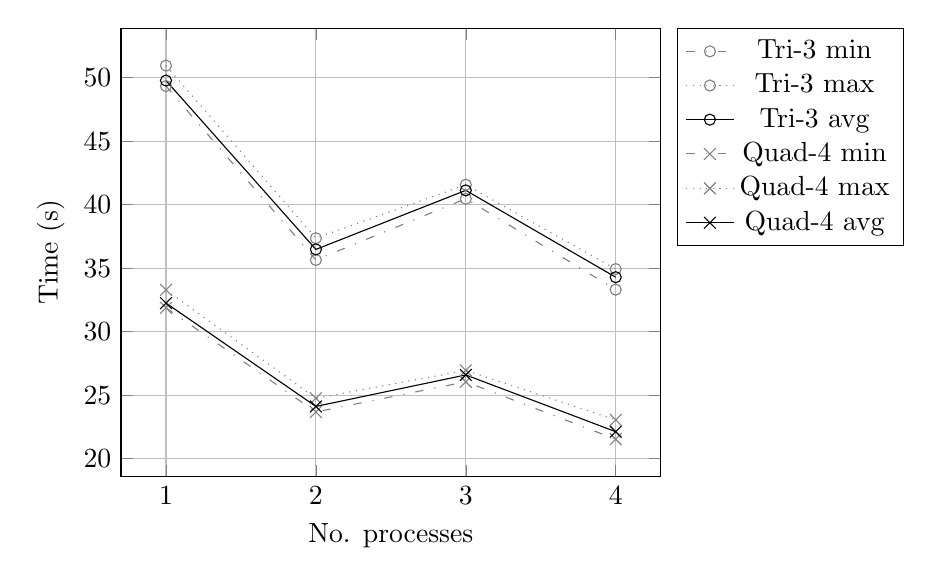
\begin{tikzpicture}
   	\begin{axis}[xlabel=No. processes,
   	ylabel=Time (s),
   	xtick={1,2,3,4},
   	ytick={50,45,40,35,30,25,20},
   	grid=major,
   	legend pos=outer north east]
   	\addplot[mark=o,loosely dashdotted,gray,mark options={solid}] plot coordinates {
   		(1,49.35)
   		(2,35.65)
   		(3,40.47)
   		(4,33.31)
   	};  
   	\addlegendentry{Tri-3 min}
   	\addplot[mark=o,dotted,gray,mark options={solid}] plot coordinates {
   		(1,50.96)
   		(2,37.36)
   		(3,41.57)
   		(4,34.93)
   	};  
   	\addlegendentry{Tri-3 max}
   	\addplot[mark=o,black] plot coordinates {
   		(1,49.78)
   		(2,36.48)
   		(3,41.13)
   		(4,34.29)
   	};  
   	\addlegendentry{Tri-3 avg}
   	%%%%%%%%%%%%%%%%%%%%%%%%%%%%%%%%%%%%%%%%%%%%%%%%%%%%%%%%%	
   	\addplot[mark=x,loosely dashdotted,gray,mark options={scale=1.5,solid}] plot coordinates {
   		(1,31.88)
   		(2,23.67)
   		(3,26.05)
   		(4,21.53)
   	};
   	\addlegendentry{Quad-4 min}
   	\addplot[mark=x,dotted,gray,mark options={scale=1.5,solid}] plot coordinates {
   		(1,33.29)
   		(2,24.75)
   		(3,26.95)
   		(4,23.05)
   	};
   	\addlegendentry{Quad-4 max}
   	\addplot[mark=x,black,mark options={scale=1.5}] plot coordinates {
   		(1,32.25)
   		(2,24.11)
   		(3,26.59)
   		(4,22.12)
   	};
   	\addlegendentry{Quad-4 avg}
   	\end{axis}
   	\end{tikzpicture}
   	\caption{Solver Times}
   	\label{fig:solver-times}
   \end{figure}
   
   \begin{figure}[htbp]
   	\centering
   	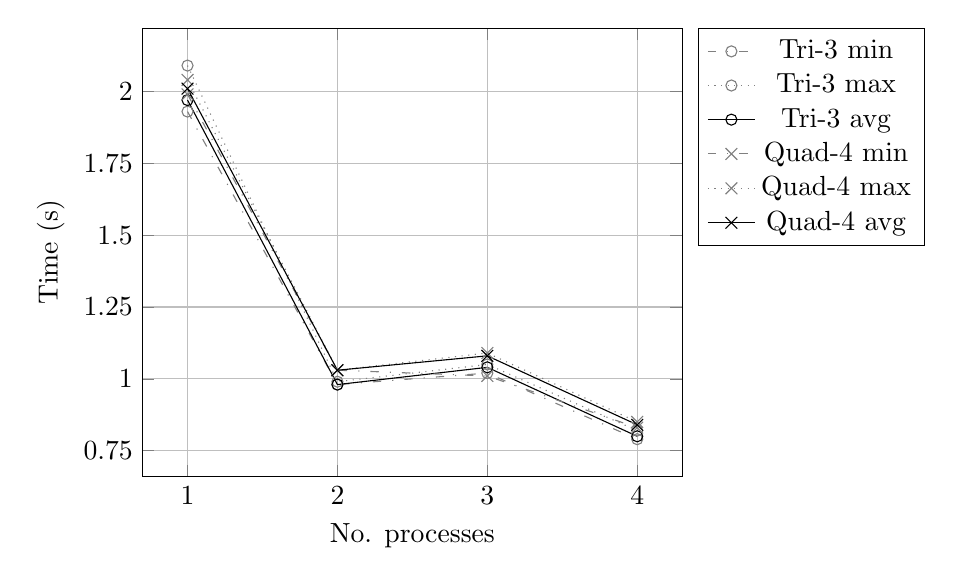
\begin{tikzpicture}
   	\begin{axis}[xlabel=No. processes,
   	ylabel=Time (s),
   	xtick={1,2,3,4},
   	ytick={2,1.75,1.5,1.25,1,0.75},
   	grid=major,
   	legend pos=outer north east]
   	\addplot[mark=o,loosely dashdotted,gray,mark options={solid}] plot coordinates {
   		(1,1.93)
   		(2,0.98)
   		(3,1.02)
   		(4,0.79)
   	};  
   	\addlegendentry{Tri-3 min}
   	\addplot[mark=o,dotted,gray,mark options={solid}] plot coordinates {
   		(1,2.09)
   		(2,0.99)
   		(3,1.05)
   		(4,0.82)
   	};  
   	\addlegendentry{Tri-3 max}
   	\addplot[mark=o,black] plot coordinates {
   		(1,1.97)
   		(2,0.98)
   		(3,1.04)
   		(4,0.8)
   	};  
   	\addlegendentry{Tri-3 avg}
   	%%%%%%%%%%%%%%%%%%%%%%%%%%%%%%%%%%%%%%%%%%%%%%%%%%%%%%%%%	
   	\addplot[mark=x,loosely dashdotted,gray,mark options={scale=1.5,solid}] plot coordinates {
   		(1,1.99)
   		(2,1.03)
   		(3,1.01)
   		(4,0.83)
   	};
   	\addlegendentry{Quad-4 min}
   	\addplot[mark=x,dotted,gray,mark options={scale=1.5,solid}] plot coordinates {
   		(1,2.04)
   		(2,1.03)
   		(3,1.09)
   		(4,0.85)
   	};
   	\addlegendentry{Quad-4 max}
   	\addplot[mark=x,black,mark options={scale=1.5}] plot coordinates {
   		(1,2.01)
   		(2,1.03)
   		(3,1.08)
   		(4,0.84)
   	};
   	\addlegendentry{Quad-4 avg}
   	\end{axis}
   	\end{tikzpicture}
   	\caption{Assembly Times}
   	\label{fig:assembly-times}
   \end{figure}
   
   \begin{figure}[htbp]
   	\centering
   	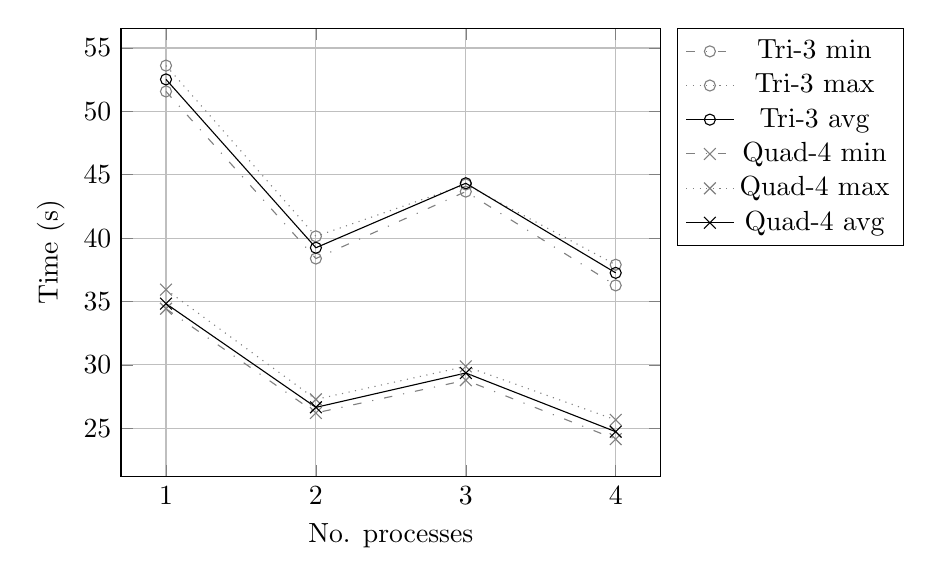
\begin{tikzpicture}
   	\begin{axis}[xlabel=No. processes,
   	ylabel=Time (s),
   	xtick={1,2,3,4},
   	ytick={55,50,45,40,35,30,25},
   	grid=major,
   	legend pos=outer north east]
   	\addplot[mark=o,loosely dashdotted,gray,mark options={solid}] plot coordinates {
   		(1,51.57)
   		(2,38.39)
   		(3,43.67)
   		(4,36.27)
   	};  
   	\addlegendentry{Tri-3 min}
   	\addplot[mark=o,dotted,gray,mark options={solid}] plot coordinates {
   		(1,53.61)
   		(2,40.14)
   		(3,44.23)
   		(4,37.90)
   	};  
   	\addlegendentry{Tri-3 max}
   	\addplot[mark=o,black] plot coordinates {
   		(1,52.52)
   		(2,39.24)
   		(3,44.33)
   		(4,37.26)
   	};  
   	\addlegendentry{Tri-3 avg}
   	%%%%%%%%%%%%%%%%%%%%%%%%%%%%%%%%%%%%%%%%%%%%%%%%%%%%%%%%%	
   	\addplot[mark=x,loosely dashdotted,gray,mark options={scale=1.5,solid}] plot coordinates {
   		(1,34.43)
   		(2,26.21)
   		(3,28.79)
   		(4,24.14)
   	};
   	\addlegendentry{Quad-4 min}
   	\addplot[mark=x,dotted,gray,mark options={scale=1.5,solid}] plot coordinates {
   		(1,35.94)
   		(2,27.28)
   		(3,29.88)
   		(4,25.66)
   	};
   	\addlegendentry{Quad-4 max}
   	\addplot[mark=x,black,mark options={scale=1.5}] plot coordinates {
   		(1,34.83)
   		(2,26.65)
   		(3,29.36)
   		(4,24.73)
   	};
   	\addlegendentry{Quad-4 avg}
   	\end{axis}
   	\end{tikzpicture}
   	\caption{Overall Times}
   	\label{fig:overall-times}
   \end{figure}
 \subsection{Test H: Coupled ``Bending Tower''}\label{sec:valid-H}
  
\newpage